%!TEX TS-program = xelatex  
%!TEX encoding = UTF-8 Unicode  

\documentclass[12pt]{article}  
\usepackage{geometry}  
\geometry{letterpaper}  
\usepackage{fancyhdr}
\usepackage{extramarks}
\usepackage{amsmath}
\usepackage{amsthm}
\usepackage{amsfonts}
\usepackage{tikz}
\usepackage[plain]{algorithm}
\usepackage{algpseudocode} 
\usepackage{caption}
\usepackage{booktabs}
\usepackage{graphics}

\usepackage{xltxtra,fontspec,xunicode}
\usepackage[slantfont,boldfont]{xeCJK}
\setCJKmainfont{宋体}   
\setmainfont{Optima}   
\defaultfontfeatures{Mapping=tex-text}  

\usepackage{xltxtra,fontspec,xunicode}
\usepackage[slantfont,boldfont]{xeCJK}
\setCJKmainfont{宋体}   
\setmainfont{Optima}   
\defaultfontfeatures{Mapping=tex-text}  

\XeTeXlinebreaklocale “zh”  
\XeTeXlinebreakskip = 0pt plus 1pt minus 0.1pt   
 
\usepackage{listings}
\usepackage{color}
\definecolor{dkgreen}{rgb}{0,0.6,0}
\definecolor{gray}{rgb}{0.5,0.5,0.5}
\definecolor{mauve}{rgb}{0.58,0,0.82}

\lstset{frame=tb,
  language=Java,
  aboveskip=3mm,
  belowskip=3mm,
  showstringspaces=false,
  columns=flexible,
  basicstyle={\small\ttfamily},
  numbers=none,
  numberstyle=\tiny\color{gray},
  keywordstyle=\color{blue},
  commentstyle=\color{dkgreen},
  stringstyle=\color{mauve},
  breaklines=true,
  breakatwhitespace=true,
  tabsize=3
} 

\topmargin=-0.45in
\evensidemargin=0in
\oddsidemargin=0in
\textwidth=6.5in
\textheight=9.0in
\headsep=0.25in

\linespread{1.1}

\pagestyle{fancy}
\lhead{\hmwkAuthorName}
\rhead{\hmwkClass}
\chead{\hmwkTitle}

\renewcommand\headrulewidth{0.4pt}
\renewcommand\footrulewidth{0.4pt}

\setlength\parindent{0pt}

% Homework Details

\newcommand{\hmwkTitle}{homework\ \#1}
\newcommand{\hmwkClass}{Deep Reinforcement Learning}
\newcommand{\hmwkAuthorName}{Tianxiao Hu}


\begin{document}
\pagebreak

\section{Question 2.2}
\begin{table}[!h]
\begin{tabular}{@{}c|cccc@{}}
\toprule
task   & mean-expert & mean-behavioral cloning & std-expert & std-behavioral cloning \\ \midrule
Ant    & 4831.49     & 4612.72                 & 121.63     & 93.05                  \\
Hopper & 3779.38     & 4.38                    & 781.79     & 117.69                              \\ \bottomrule
\end{tabular}
\caption{Results for comparison of task {\bf Ant} and {\bf Hopper}. With {\em rollouts} $= 20$ and {\em epochs} $ = 10$. Two four-layer fully-connected network ares trained in behavioral cloning. The first 3 layers have 128 nodes and the amount of nodes in the output layer is the dimension of action.}
\end{table}

\section{Question 2.3}

\begin{figure}[!h]
\centering
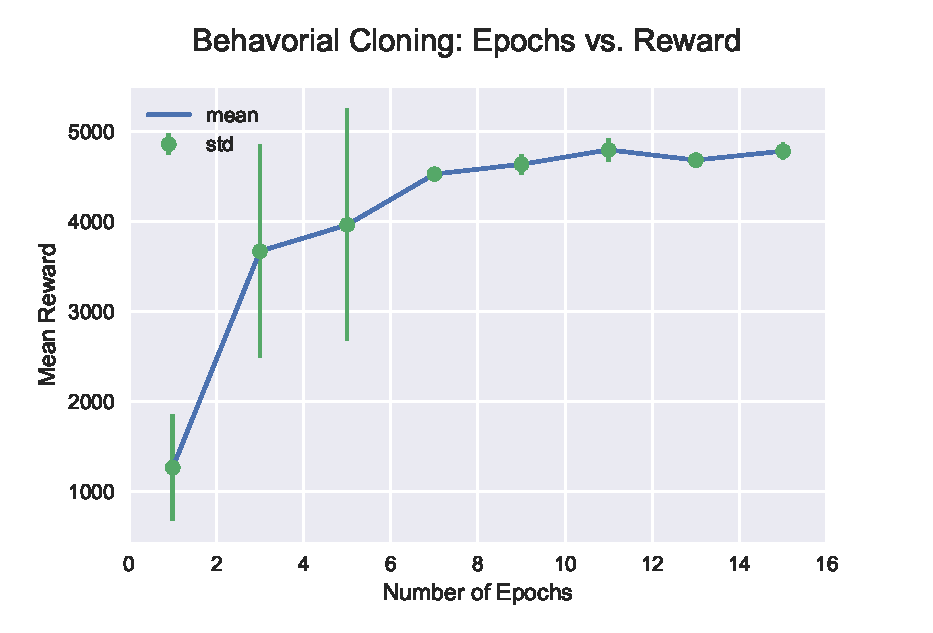
\includegraphics[width=5in]{2-2.eps}
\caption{Figure 1 shows how the number of {\em epochs} affects the performance of the behavioral cloning agent. Experiments was performed on task {\bf Ant}. As the number of {\em epochs} goes up, the mean {\em reward} is going up as well. That's because training more epochs makes the neural network to fit the dataset better, thus improves the performance of the agent.}
\end{figure}

\newpage

\section{Question 3.2}
\begin{figure}[!h]
\centering
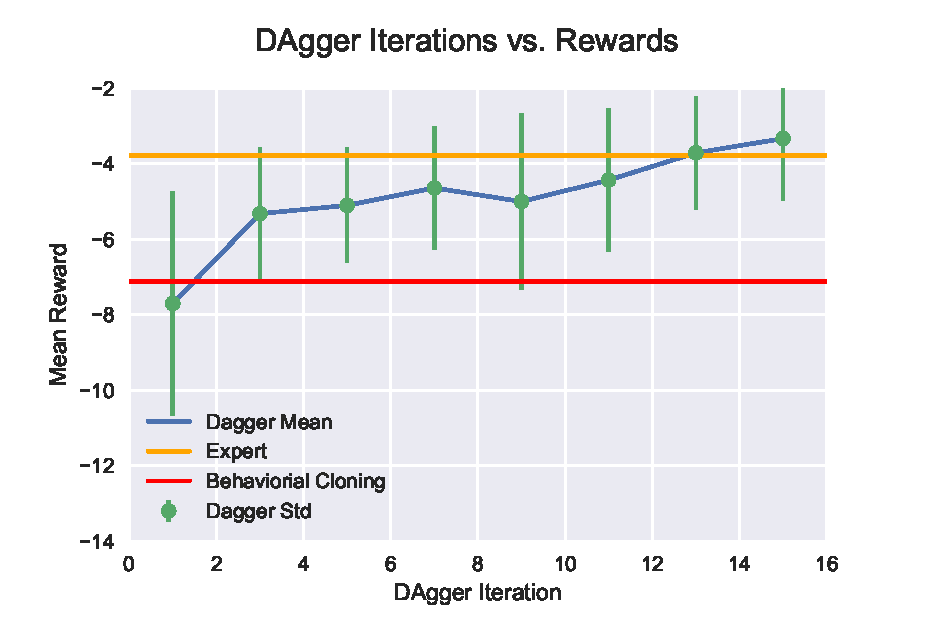
\includegraphics[width=5in]{3-2.eps}
\caption{Figure 2 shows how the number of {\em iterations} affects the performance of the Dagger agent. Experiments was performed on task {\bf Reacher}. The network structure and dataset are totally same as stated in Quesion 2.2(four-layer fully-connected network and {\em rollouts} $= 20$). As the number of {\em iterations} goes up, the mean {\em reward} is going up as well. That's because more {\em iterations} makes the Dagger agent fit the training data better and eventually outperforms the expert policy.}
\end{figure}

\end{document}  
  